\documentclass[conference]{IEEEtran}
\usepackage[utf8]{inputenc}
\usepackage[T1]{fontenc}
\usepackage{amsmath,amssymb}
\usepackage{graphicx}
\usepackage{booktabs}
\usepackage{listings}
\usepackage{xcolor}
\usepackage{hyperref}
\usepackage{cite}
\hypersetup{colorlinks=true,linkcolor=black,citecolor=black,urlcolor=blue}
\lstset{basicstyle=\ttfamily\scriptsize,breaklines=true,frame=single,columns=fullflexible,
        commentstyle=\color{gray},keywordstyle=\bfseries,language=C++}

\title{Economic Dispatch and DC Optimal Power Flow with Wind Integration:\\
       an Active-Set KKT Solver with a natID Front End}

\author{\IEEEauthorblockN{Faris Muratovi\'c}
\IEEEauthorblockA{Project Report (Numerical Optimization, Topic~11)\\
Student ID: 19958\\
Faculty of Electrical Engineering, University of Sarajevo\\
Instructor: Prof.\ Dr.\ Izudin D\v{z}afi\'c}}

\begin{document}
\maketitle

\begin{abstract}
This project implements economic dispatch (ED) and DC optimal power flow (DC-OPF) from first principles. The optimality conditions of the quadratic-cost dispatch problem are written out as a Karush--Kuhn--Tucker (KKT) system, inequality constraints on generator output and line flow are handled by an active-set method, wind is injected as a zero-marginal-cost source, and transmission losses are modelled by successive linearisation. The KKT system is an indefinite saddle-point system with structural zeros on its diagonal; it is solved with the pivoting sparse LU solver of the natID framework, and every solve is residual-checked. Correctness is established by a 56-check validation suite: the DC-OPF solution reduces exactly to ED when no transmission constraint binds, the congested two-bus case reproduces an independent hand derivation to every printed digit, and the locational marginal price splits by exactly the congestion price. A four-tab desktop application built with natGUI exposes the solver interactively: a results dashboard with scenario presets, a parameter panel, an annotated five-bus network schematic and the four deliverable charts, all exportable to PDF. On the five-bus test system, 30\,\% wind penetration reduces fuel cost by a third but slightly \emph{increases} network losses, because the wind resource is electrically distant from the load.
\end{abstract}

\begin{IEEEkeywords}
economic dispatch, DC optimal power flow, KKT conditions, active-set method, locational marginal price, wind integration, transmission losses, sparse LU, natID
\end{IEEEkeywords}

\section{Introduction}
Economic dispatch is the classical problem of sharing a given electrical load among thermal generators so that total fuel cost is minimal. Its network-aware generalisation, optimal power flow, adds the physics of the transmission grid: power must balance at every bus, and no line may carry more than its rating. Under the standard DC approximation the flow equations become linear in the bus voltage angles, and the whole problem becomes a convex quadratic program whose optimality conditions are a single linear system per active set. That makes it an ideal vehicle for a numerical-optimization project: the mathematics is small enough to derive by hand, the solutions can be checked analytically, and yet the linear algebra has a genuine trap (an indefinite matrix with a zero diagonal) that punishes a naive solver.

The project deliverables are (i) a solver library \texttt{core} that implements ED and DC-OPF with generator bounds, line limits, wind injection and a loss model; (ii) a console driver \texttt{cli} that runs the validation suite and writes CSV data for the figures; and (iii) a graphical application \texttt{dispatchGui} written against the natID framework, which allows the parameters to be edited, the case solved, and the results inspected on a dashboard, a network schematic and four analytical charts. All three targets share one CMake build and compile on Windows, macOS and Linux.

\section{Problem Statement}
\subsection{Economic dispatch}
Each thermal generator $i$ has a quadratic fuel cost in its active power output $P_i$,
\begin{equation}
  C_i(P_i) = a_i P_i^2 + b_i P_i + c_i,\qquad a_i > 0 .
\end{equation}
Economic dispatch minimises the total cost subject to a single system-wide balance equation and box constraints:
\begin{equation}
  \min_P \sum_i C_i(P_i)\quad\text{s.t.}\quad \sum_i P_i = D,\quad P_i^{\min}\le P_i \le P_i^{\max}.
  \label{eq:ed}
\end{equation}
Its well-known solution is the \emph{equal incremental cost} rule: every free generator runs at the output where $\mathrm{d}C_i/\mathrm{d}P_i = 2a_iP_i+b_i$ equals the common system marginal price $\lambda$.

\subsection{DC optimal power flow}
DC-OPF replaces the single balance equation by one per bus and adds line-flow limits:
\begin{align}
  \min_{P,\theta}\ &\sum_i C_i(P_i) \label{eq:opf}\\
  \text{s.t.}\ & \sum_{g\in i} P_g - \sum_j B_{ij}\theta_j = D_i \quad \forall\ \text{bus } i, \nonumber\\
  & |B_l(\theta_{\mathrm{from}}-\theta_{\mathrm{to}})| \le F_l^{\max} \quad \forall\ \text{line } l, \nonumber\\
  & P_i^{\min}\le P_i\le P_i^{\max},\qquad \theta_{\mathrm{slack}} = 0. \nonumber
\end{align}
Here $\theta$ is the vector of bus voltage angles and $\mathbf{B}$ is the susceptance matrix, $B_{ij}=-1/x_{ij}$ off the diagonal and $B_{ii}=\sum 1/x$ over the lines touching bus $i$. The DC model is the linearisation of the AC power-flow equations under the assumptions that voltage magnitudes are close to 1~p.u.\ and angle differences across lines are small; the flow on a line is then proportional to the angle difference divided by the reactance.

Two extensions are implemented. \textbf{Wind} is injected at a designated bus as a zero-marginal-cost source that reduces the demand the thermal units must cover there; the installed capacity is 150~MW and a \emph{wind fraction} $w\in[0,1]$ selects how much of it is available. \textbf{Losses} are modelled per line as $g_l(\Delta\theta_l)^2$ with $g_l = r_l/(r_l^2+x_l^2)$, half of each line's loss being injected as additional demand at each of its end buses.

\section{Method}
\subsection{KKT formulation}
Forming the Lagrangian of \eqref{eq:opf} and differentiating gives three families of stationarity conditions that are assembled into one linear system per active-set iteration. For every free generator the marginal cost equals the price \emph{at its own bus},
\begin{equation}
  2a_gP_g + b_g = \lambda_{\mathrm{bus}(g)} ,
\end{equation}
for every non-slack bus the prices satisfy a network equation,
\begin{equation}
  (\mathbf{B}\lambda)_k + \sum_{l\ \text{active}} \pm B_l\,\mu_l = 0 ,
\end{equation}
and these are completed by the per-bus balance equations and one equality per binding line that pins its flow at the limit. The unknown vector is
\[
  x = \bigl[\,P_{\text{free}} \mid \theta_{\text{non-slack}} \mid \lambda_{\text{all buses}} \mid \mu_{\text{binding lines}}\,\bigr] ,
\]
which for $N$ buses, $n_g$ generators and $n_a$ active lines has $n_g+(N-1)+N+n_a$ entries, matched exactly by the number of equations.

Two points were the source of real difficulty during implementation and are recorded here because they are easy to get wrong. First, $\theta$ and $\lambda$ are different objects: $\theta$ is a primal variable in the physical flow equations while $\lambda$ is the dual variable (the locational marginal price) of the balance constraint. An early version conflated them and produced a system that looked plausible and was wrong. Second, the KKT matrix is \emph{not symmetric}: the $P$--$\lambda$ coupling has coefficient $-1$ in the cost block but $+1/S_{\mathrm{base}}$ in the balance block, because $P$ is in MW in the cost equations and in per-unit in the balance equations. Declaring the matrix symmetric and supplying only one triangle makes the factorisation fail outright.

\subsection{Active-set method}
Generator bounds and line limits are handled by an active-set scheme. Starting from an empty active set, the equality-constrained KKT system is solved, the result is checked against every inequality, and the \emph{single worst violation} is added to the active set before re-solving. Adding one constraint per iteration matters: an earlier version added every violated constraint from one intermediate solve, but because intermediate iterates are themselves infeasible this cascades, and in the five-bus case ended with all six lines pinned simultaneously---more equality constraints than the network has degrees of freedom, hence a singular system. Generator bounds and line limits are not independent either (pinning a line changes every generator output and vice versa), so both families are re-checked after every single activation. If an activation makes the system unsolvable it is reverted and the search stops at the last feasible iterate.

\subsection{Losses by successive linearisation}
Pure DC-OPF is lossless by construction. The loss model is therefore an outer iteration: solve the lossless problem, compute each line's loss from the resulting angles, re-inject half of each loss as extra demand at each end bus, and repeat until the injections stop changing. Convergence is fast---five outer iterations to a tolerance of $10^{-4}$~MW on the test system (Table~\ref{tab:loss}).

\subsection{Linear algebra}
The KKT system is an indefinite saddle-point system: the $\lambda$ and $\mu$ rows have no diagonal entries, so the matrix has structural zeros on the diagonal. \texttt{dense::Matrix::solve} was used first; it reports success while returning a solution with a residual of order $10^2$, i.e.\ it silently does not solve the system. The final implementation uses natID's \texttt{sparse::createDblSolver} with \texttt{Symmetry::NonSymmetric}, \texttt{SolverType::LU} and \texttt{Pivoting::DiagonalMultiPass}, which handles the zero diagonal correctly. Because a direct solver can fail silently on such a system, every solve is followed by an explicit residual check: $\mathbf{A}x$ is recomputed from the stored triplets and compared with $b$, and a residual above $10^{-4}$ is treated as infeasible rather than trusted. This check is what made the original failure visible and it is retained permanently.

\begin{lstlisting}[caption={Active-set loop (abridged from \texttt{OPFSolver.cpp}).},label=lst:as]
OPFResult OPFSolver::solve(const Network& net,
        const std::vector<Generator>& gens, double windFrac) const
{
    ActiveSet active;                       // empty at start
    for (int it = 0; it < maxIter; ++it) {
        KKT kkt = assemble(net, gens, windFrac, active);
        if (!kkt.solveAndCheckResidual(1e-4))  // pivoting sparse LU
            { active.revertLast(); break; }
        Violation v = worstViolation(kkt, net, gens);
        if (!v.found) return kkt.result();  // KKT point is feasible
        active.add(v);                       // one constraint per pass
    }
    return lastFeasible;
}
\end{lstlisting}

\section{Test Systems}
\subsection{Two-bus system (analytically verifiable)}
Two generators, a 500~MW load at bus~1 and one line with $x=0.10$~p.u. G1 (bus~0, slack) has $a=0.008$, $b=8.0$, $50\le P\le 300$; G2 (bus~1) has $a=0.009$, $b=6.4$, $50\le P\le 400$. The case is small enough that every quantity can be derived by hand.

\subsection{Five-bus system}
Table~\ref{tab:5bus} lists the five-bus network used for every other experiment and by the application. $S_{\mathrm{base}}=100$~MVA; the 500~MW load is at bus~3 and the 150~MW wind farm at bus~4. The loop closed by L5 means the flow split is decided by the optimisation rather than forced by topology, and L4 is deliberately tight: the unconstrained optimum pushes 321.7~MW through it.

\begin{table}[t]
\caption{Five-bus test system.}
\label{tab:5bus}
\centering
\begin{tabular}{@{}lccccc@{}}
\toprule
Generator & Bus & $a$ & $b$ & $P^{\min}$ & $P^{\max}$ \\
\midrule
G1 & 0 (slack) & 0.008 & 8.0 & 50 & 300 \\
G2 & 1 & 0.009 & 6.4 & 50 & 400 \\
G3 & 2 & 0.007 & 7.9 & 30 & 350 \\
\bottomrule
\end{tabular}
\vspace{4pt}

\begin{tabular}{@{}lccc@{}}
\toprule
Line & From--To & $x$ (p.u.) & Limit (MW) \\
\midrule
L0 & 0--1 & 0.10 & 250 \\
L1 & 0--4 & 0.15 & 150 \\
L2 & 1--2 & 0.10 & 200 \\
L3 & 4--2 & 0.12 & 150 \\
\textbf{L4} & \textbf{2--3} & \textbf{0.08} & \textbf{180} \\
L5 & 1--3 & 0.20 & 200 \\
\bottomrule
\end{tabular}
\end{table}

\section{Software Architecture}
The code is organised as a static library and three front ends that share one CMake build (Fig.~\ref{fig:arch}).

\begin{figure}[t]
\centering
\begin{lstlisting}[frame=none,basicstyle=\ttfamily\scriptsize]
DSAI-NO-Project/
  core/     Network, Generator, OPFSolver, DispatchSolver,
            Sweep, TestNetwork      (static library, natID sparse)
  cli/      validation suite (56 checks) + CSV export
  gui/      main.cpp: four-tab natGUI application
  verify/   independent numerical checks
  res/      DevRes.xml, app icon
  make_figures.py, dispatch.cmake, CMakeLists.txt
\end{lstlisting}
\caption{Repository layout. Everything numerical lives in \texttt{core}; both front ends only call into it.}
\label{fig:arch}
\end{figure}

\texttt{core} exposes a small API: \texttt{Network} (buses, lines, susceptance matrix), \texttt{Generator}, \texttt{OPFSolver::solve} and \texttt{solveWithLosses} returning an \texttt{OPFResult} (dispatch, angles, per-bus $\lambda$, flows, multipliers $\mu$, losses, cost, residual, bound flags), and \texttt{Sweep} which produces the data for the demand and wind sweeps and the per-generator cost curves. The \texttt{cli} target runs the validation suite and writes five CSV files; \texttt{make\_figures.py} renders them with matplotlib.

The graphical application is built on the natID framework's \texttt{natGUI} layer. Its native widgets (numeric fields, slider, check box, combo box, buttons, tab view) are used for input, while every result is drawn on \texttt{gui::Canvas} subclasses through a small set of primitives (\texttt{Shape::drawLine}, \texttt{Shape::createPolyLine}, \texttt{DrawableString::draw}), which keeps the drawing code independent of the framework's API surface. The window is a header strip plus a \texttt{StandardTabView} with four tabs:
\begin{itemize}
  \item \textbf{Overview}: a scenario selector (Base, High wind, Low wind, High demand, Low demand, Custom), a status banner, five KPI tiles (fuel cost, total generation, wind, $\lambda$, losses), a compact dispatch chart, a network preview, the energy balance and the KKT residual, with PDF export (Fig.~\ref{fig:params}).
  \item \textbf{Parameters}: the generator table ($a,b,c,P^{\min},P^{\max}$), system demand, wind penetration, the loss toggle, Solve, and six result cards. Every edit flips the scenario to \emph{Custom}; input is validated before solving (positive $a$, $P^{\min}\le P^{\max}$, capacity versus demand).
  \item \textbf{Network}: the five-bus schematic with flow direction arrows, MW per line, generator and wind output, $\lambda$ at every bus, and lines at their limit drawn in red.
  \item \textbf{Charts}: the four deliverable charts (Fig.~\ref{fig:charts}), exportable to PDF.
\end{itemize}
The application runs the solver synchronously: a solve of the five-bus system takes well under a millisecond, and the three sweeps behind the Charts tab (21 demand points, 21 lossless and 11 lossy wind points) complete in a few milliseconds, so no worker thread is needed.

\begin{figure}[t]
\centering
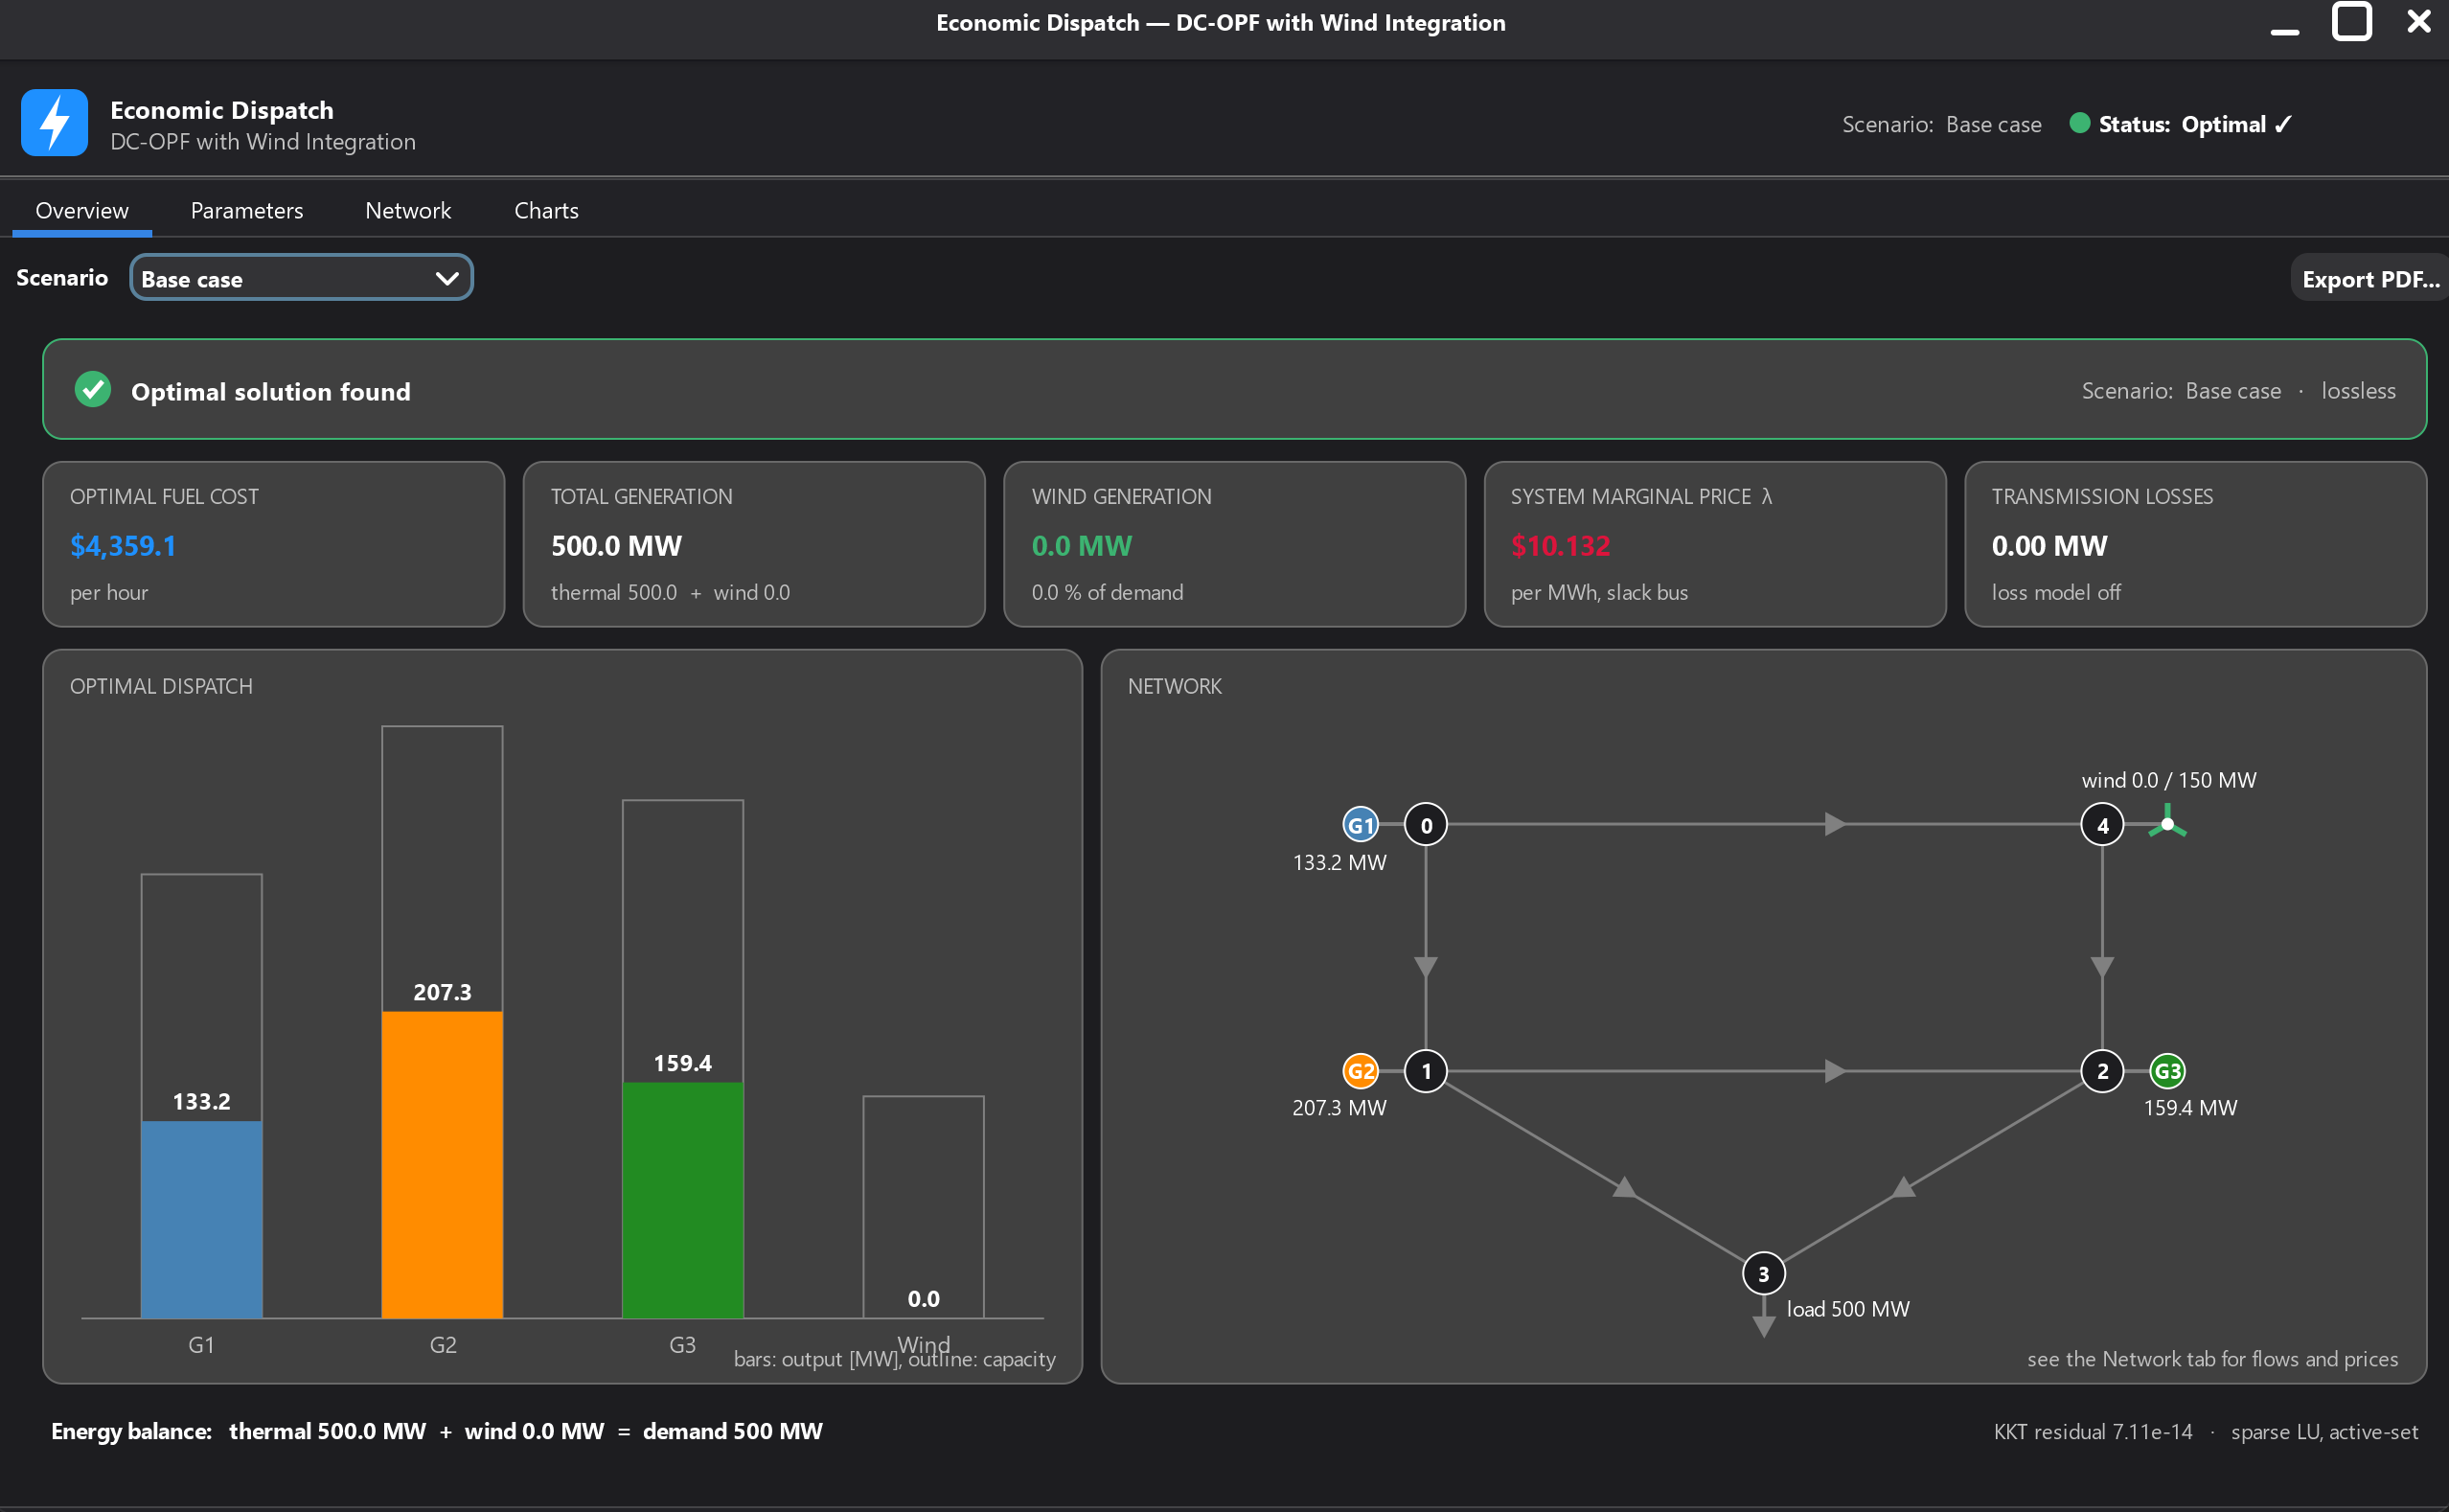
\includegraphics[width=\columnwidth]{Images/overview.png}
\caption{Overview tab after solving the base case: status banner, KPI tiles (cost, generation, wind, $\lambda$, losses), dispatch versus capacity, network preview with flow direction arrows, energy balance and KKT residual.}
\label{fig:params}
\end{figure}

\begin{figure}[t]
\centering
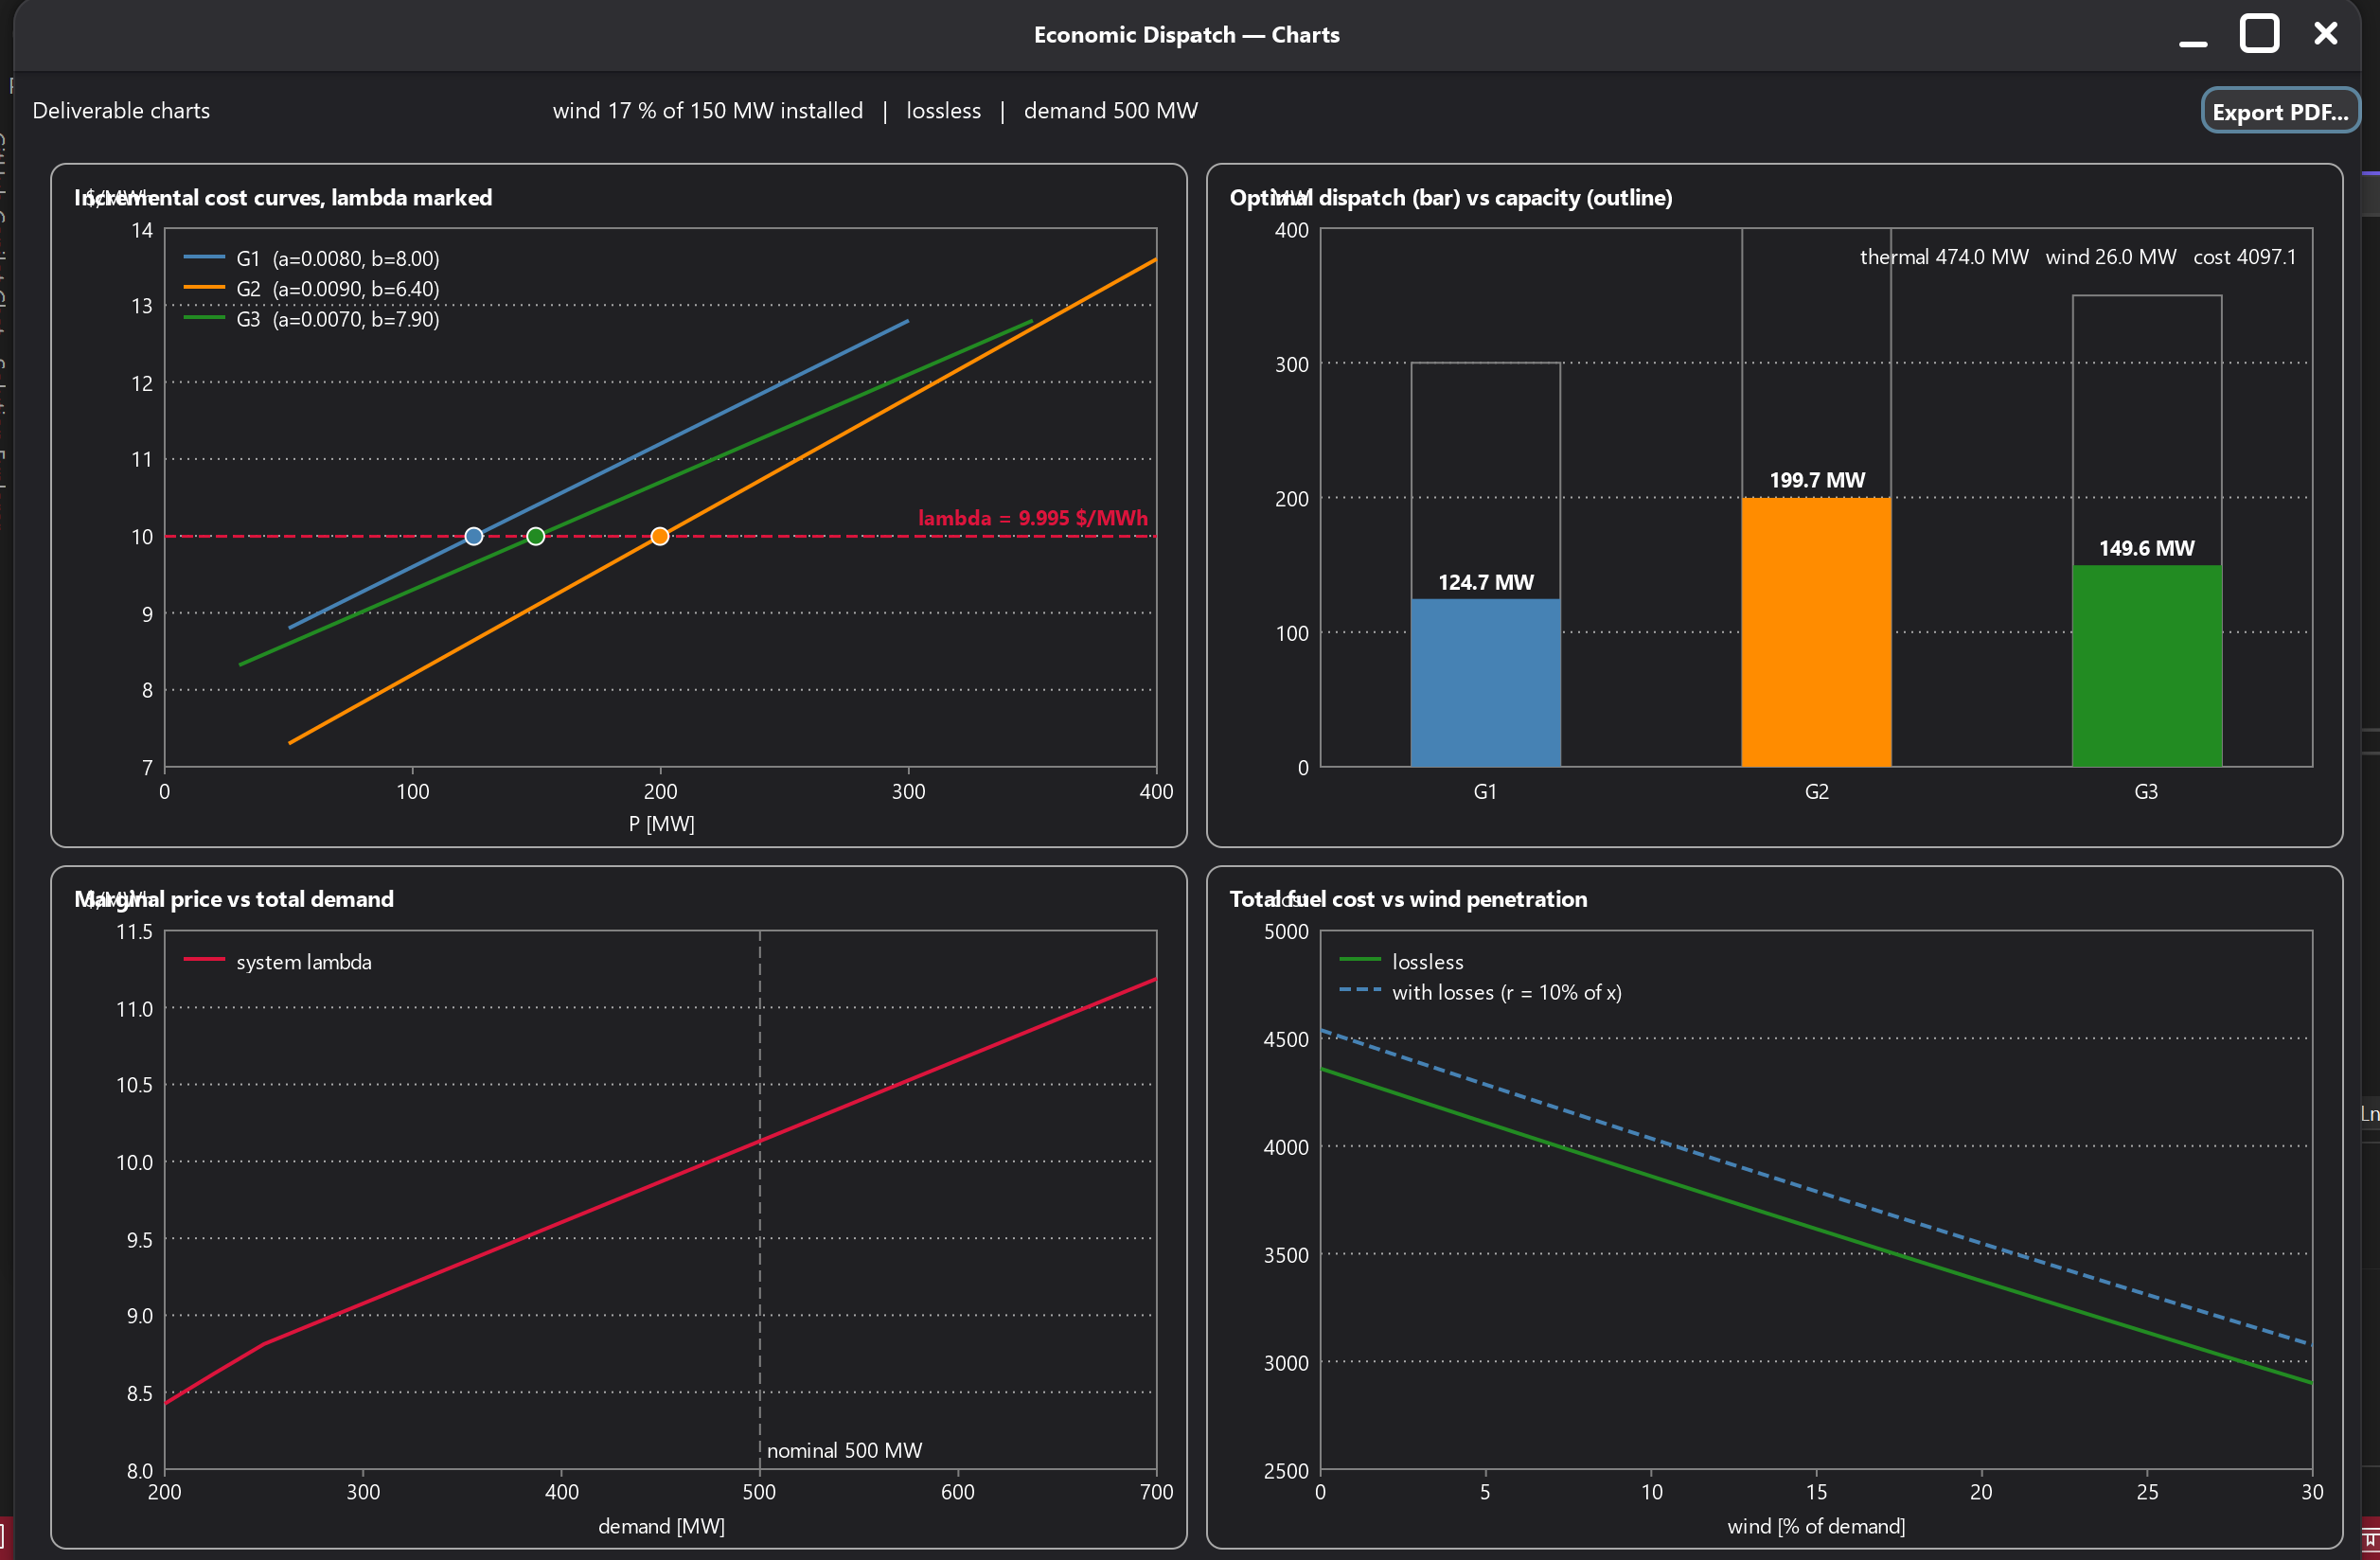
\includegraphics[width=\columnwidth]{Images/charts.png}
\caption{The four deliverable charts as drawn by the application: incremental cost curves with $\lambda$ marked, dispatch versus capacity, $\lambda$ versus demand, and cost versus wind penetration (lossless and lossy).}
\label{fig:charts}
\end{figure}

\section{Results}
All results are produced by the \texttt{cli} target and reproduced by its built-in validation suite (\textbf{56 checks, 0 failures}); the KKT residual is reported for every solve.

\subsection{Economic dispatch baseline}
Two generators, $D=500$~MW: $P_1=217.6471$~MW, $P_2=282.3529$~MW, $\lambda=11.4824$, cost 4644.7059. The equal-incremental-cost condition checks: $2(0.008)(217.6471)+8 = 11.4824$ and $2(0.009)(282.3529)+6.4=11.4824$.

\subsection{DC-OPF reduces to ED when nothing binds}
With the two-bus line unconstrained the DC-OPF result is \emph{identical} to the ED result: $P=[217.6471,\,282.3529]$, $\lambda=11.4824$ at both buses, $\theta_1=-0.2176$~rad, flow 217.6471~MW, cost 4644.7059, residual 0. This is the central correctness test: with no binding transmission constraint the network model must add nothing, and it does not. The five-bus case behaves the same way: $P=[133.2461,\,207.3298,\,159.4241]$, $\lambda=10.1319$ uniform across all five buses, cost 4359.1492, residual $5.7\times10^{-14}$, matching the three-generator ED solution exactly. A uniform $\lambda$ is the signature of an uncongested network.

\subsection{Congestion separates locational prices}
Capping the two-bus line at 100~MW, below the 217.6~MW it naturally carries, gives Table~\ref{tab:cong}. Every value matches the independent hand derivation. The cheap generator is held back by the line, the expensive one makes up the difference, cost rises from 4644.71 to 4880.00, and the price splits by exactly the congestion price $\mu=\lambda_1-\lambda_0=4.0$: the textbook mechanism by which locational marginal prices arise.

\begin{table}[t]
\caption{Congested two-bus case (line limit 100~MW). Residual $7.1\times10^{-15}$.}
\label{tab:cong}
\centering
\begin{tabular}{@{}lrr@{}}
\toprule
Quantity & Solver & Hand-derived \\
\midrule
$P_1$ & 100.0000 MW & 100 \\
$P_2$ & 400.0000 MW & 400 \\
$\lambda$ bus 0 & 9.6000 & 9.6 \\
$\lambda$ bus 1 & 13.6000 & 13.6 \\
flow & 100.0000 MW & 100 (at limit) \\
$\mu$ (congestion price) & 4.0000 & $\lambda_1-\lambda_0 = 4.0$ \\
total cost & 4880.0000 & --- \\
\bottomrule
\end{tabular}
\end{table}

\subsection{Generator bounds bind correctly}
With G2's capacity reduced to 100~MW the active-set method detects the 107.33~MW violation, pins G2 at its maximum and re-solves: $P=[183.3333,\,100.0000,\,216.6667]$~MW, $\lambda=10.9333$ uniform, cost 4505.8333, residual $2.8\times10^{-14}$. Generation still meets demand exactly, both free generators stay within their bounds, and the price rises from 10.1319 to 10.9333 because cheap capacity has been withdrawn.

\subsection{Wind displaces thermal generation}
Table~\ref{tab:wind} shows the five-bus system with line limits relaxed to isolate the wind effect. Thermal output falls one-for-one with wind injection and both $\lambda$ and total cost fall monotonically: zero-marginal-cost wind displaces the most expensive thermal increment first. Over the 21-point sweep the cost falls from 4359.15 to 2898.73, a 33.5\,\% reduction at 30\,\% penetration.

\begin{table}[t]
\caption{Wind sweep, lossless, line limits relaxed.}
\label{tab:wind}
\centering
\begin{tabular}{@{}rrrrr@{}}
\toprule
Wind avail. & Injected & Thermal & $\lambda$ & Cost \\
\midrule
0\,\% & 0 MW & 500.00 MW & 10.1319 & 4359.15 \\
50\,\% & 75 MW & 425.00 MW & 9.7361 & 3614.10 \\
100\,\% & 150 MW & 350.00 MW & 9.3403 & 2898.73 \\
\bottomrule
\end{tabular}
\end{table}

\subsection{Transmission losses}
With $r=10\,\%$ of $x$ on every line the outer loss iteration converges in five passes (Table~\ref{tab:loss}). At convergence $P=[139.0491,\,212.4881,\,166.0561]$~MW; total generation $517.5933$~MW equals the 500~MW demand plus $17.5933$~MW of losses exactly; cost is 4538.22 versus 4359.15 lossless, so losses add 4.1\,\% to the fuel bill; and $\lambda$ rises from 10.1319 to 10.2248, correctly reflecting that serving one more MW of load now also requires covering its marginal losses.

\begin{table}[t]
\caption{Convergence of the loss iteration.}
\label{tab:loss}
\centering
\begin{tabular}{@{}crr@{}}
\toprule
Iteration & Total loss (MW) & Change \\
\midrule
0 & 17.0179 & 7.2467 \\
1 & 17.5767 & 0.2121 \\
2 & 17.5928 & 0.0062 \\
3 & 17.5933 & $1.8\times10^{-4}$ \\
4 & 17.5933 & $5.4\times10^{-6}$ \\
\bottomrule
\end{tabular}
\end{table}

\subsection{Losses versus wind penetration}
Fig.~\ref{fig:windsweep} plots cost and losses against wind penetration with the loss model active. Losses \emph{increase} by about 7\,\% across the range (17.59 to 18.87~MW) rather than decreasing as one might expect from reduced thermal output. The reason is locational: the wind bus~4 is electrically distant from the load at bus~3, reachable only through L3 and L4. Displacing nearby thermal generation with distant wind lengthens the average path power travels, and the quadratic loss term grows faster with flow than the reduction in thermal output reduces it. The economic benefit of the wind resource (cost down 32\,\%) is unambiguous, but its effect on losses depends on \emph{where} it is connected, not just how much it produces---an argument for treating siting as part of the optimisation.

\begin{figure}[t]
\centering
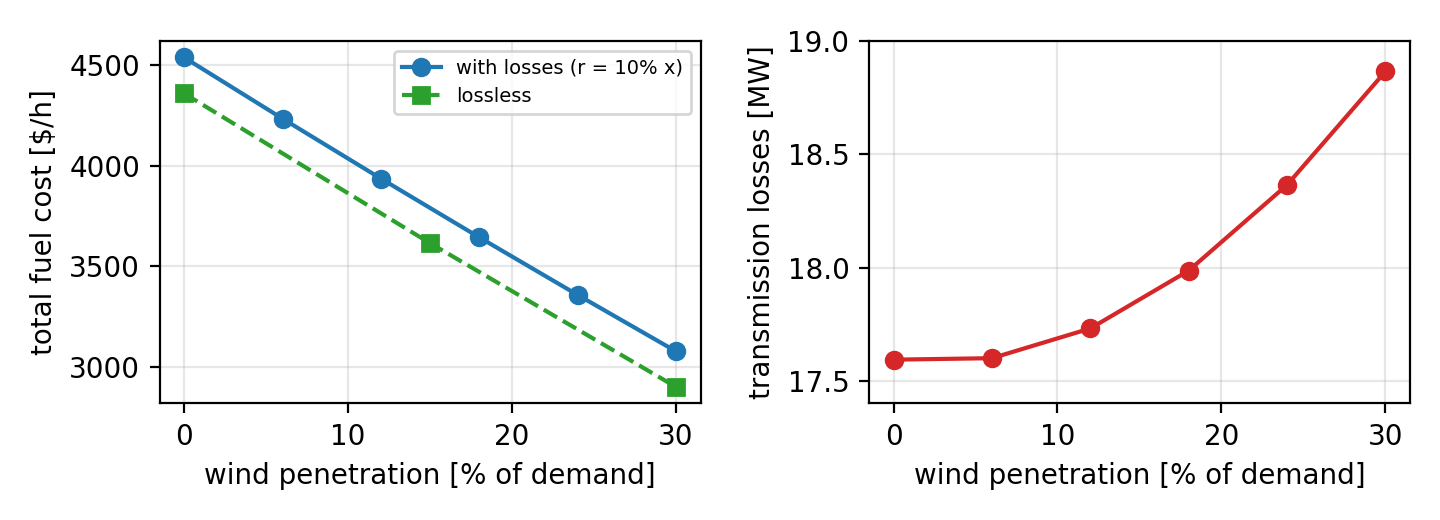
\includegraphics[width=\columnwidth]{Images/wind_sweep.png}
\caption{Total fuel cost (left) and transmission losses (right) versus wind penetration on the five-bus system.}
\label{fig:windsweep}
\end{figure}

\subsection{Interactive scenarios}
The application's scenario presets exercise the same solver on the same network. At 17\,\% wind availability (Fig.~\ref{fig:charts}) the dispatch is $P=[124.7,\,199.7,\,149.6]$~MW with 26.0~MW of wind, $\lambda=9.995$, cost 4097.1; at 80.8\,\% it is $[93.3,\,171.8,\,113.7]$~MW with 121.2~MW of wind, $\lambda=9.492$, cost 3169.73; the base case (Fig.~\ref{fig:params}) gives $[133.2,\,207.3,\,159.4]$~MW, $\lambda=10.132$ and cost 4359.1, matching the validation suite. In every case the three incremental-cost curves cross the $\lambda$ line exactly at the dispatched outputs, which is the equal-incremental-cost condition made visible, and the $\lambda$-versus-demand chart shows the price rising from 8.43 to 11.19 over the $0.4\times$--$1.4\times$ demand sweep.

\section{Portability}
The project is built with CMake against the natID SDK. The numerical code uses only the C++20 standard library and natID's \texttt{mainUtils}/\texttt{Matrix} libraries, and compiles without warnings under MSVC and GCC. The two platform-specific points are confined to the build files: the GUI executable is a \texttt{/SUBSYSTEM:WINDOWS} application on Windows (\texttt{gui/WinMain.h} redirects the entry point to \texttt{main}), and the name of the Matrix library is derived from the framework's own \texttt{mainUtils} path so that the \texttt{.lib}/\texttt{.dylib}/\texttt{.so} convention of each platform is followed automatically.

\section{Limitations and Future Work}
\textbf{Simultaneous multi-constraint active sets.} The method activates one constraint at a time and reverts an activation that makes the system unsolvable. It does not implement constraint dropping (removing a constraint whose multiplier has the wrong sign) or detection of linear dependence among candidate constraints. In the five-bus case, pinning L4 alone produces a mathematically exact solution (residual $2.3\times10^{-13}$) in which G3 is dispatched to $-547$~MW---a valid solution of the stated equalities but not a physical one. Reaching a physical solution requires a generator bound to bind simultaneously, and the combination of L4, L2 and two generator bounds turns out to be over-determined for this topology. Constraint-dependency detection is the natural next step; the application therefore runs its scenarios with line limits relaxed, as the validation suite does.

\textbf{Degenerate (linear) costs.} The formulation assumes $a>0$. With linear costs and two generators at one bus the stationarity conditions demand that the bus price equal two different constants at once; such problems are linear programs with corner solutions and need a simplex or interior-point method. This was confirmed on the published PJM five-bus benchmark, whose data uses linear costs.

\textbf{DC approximation and loss model.} Voltage magnitudes and reactive power are outside the model by construction; angle differences in the test cases reach 0.43~rad, at the edge of where the small-angle assumption is comfortable. Losses enter only through the outer iteration and not through the stationarity conditions, so the lossy result is a fixed point rather than a true optimum of the lossy problem.

\section{Conclusion}
The project implements economic dispatch and DC-OPF from first principles via the KKT conditions, with an active-set treatment of generator bounds and line limits, extended with wind injection and a quadratic loss model, and wraps the solver in a portable natID desktop application. Correctness is established by a 56-check validation suite: DC-OPF reduces exactly to ED when no transmission constraint binds, the congested two-bus case reproduces an independent hand derivation to every printed digit, and every linear solve is residual-checked. Two findings are worth carrying forward. First, the indefinite saddle-point structure of the KKT system genuinely requires a pivoting solver: a non-pivoting direct solve fails silently, returning plausible numbers with a residual of order $10^2$, which is why the residual check became a permanent part of the solver. Second, wind integration reduced fuel cost by a third but slightly increased network losses because the wind resource sits far from the load---a result that argues for treating renewable siting, not just capacity, as an optimisation variable.

\begin{thebibliography}{9}
\bibitem{wood} A. J. Wood, B. F. Wollenberg, and G. B. Shebl\'e, \emph{Power Generation, Operation, and Control}, 3rd ed. Hoboken, NJ: Wiley, 2013.
\bibitem{nocedal} J. Nocedal and S. J. Wright, \emph{Numerical Optimization}, 2nd ed. New York: Springer, 2006.
\bibitem{stott} B. Stott, J. Jardim, and O. Alsa\c{c}, ``DC power flow revisited,'' \emph{IEEE Trans. Power Syst.}, vol. 24, no. 3, pp. 1290--1300, 2009.
\bibitem{benzi} M. Benzi, G. H. Golub, and J. Liesen, ``Numerical solution of saddle point problems,'' \emph{Acta Numerica}, vol. 14, pp. 1--137, 2005.
\bibitem{natid} I. D\v{z}afi\'c, \emph{natID framework: Common/Include SDK documentation}, 2026.
\end{thebibliography}

\end{document}
